\documentclass[12pt]{report}

% --- Idioma y codificación ---
\usepackage[spanish]{babel}
\usepackage[utf8]{inputenc}

% --- Matemáticas ---
\usepackage{amsmath, amssymb, amsthm}

% --- Gráficos y figuras ---
\usepackage{graphics, graphicx, subfigure}
\usepackage{tikz, pgffor, ifthen}

% --- Tablas y estructuras ---
\usepackage{array, multicol, longtable, booktabs}

% --- Listas y enumeraciones ---
\usepackage{enumerate, enumitem}

% --- Márgenes y geometría ---
\usepackage[a4paper, margin=1.5cm]{geometry}

% --- Diseño y marco ---
\usepackage[framemethod=TikZ]{mdframed}

% --- Texto y contenido de prueba ---
\usepackage{lipsum}

\usepackage{subfiles}

% --- Hipervínculos ---
\usepackage{hyperref}
\usepackage{multirow}

\hypersetup{
    colorlinks=true,
    linkcolor=black,
    filecolor=magenta,
    urlcolor=cyan
}

% --- Código fuente (listings) ---
\usepackage{listings}
\usepackage{xcolor}

\definecolor{listing-background}{HTML}{F7F7F7}
\definecolor{listing-rule}{HTML}{B3B2B3}
\definecolor{listing-numbers}{HTML}{B3B2B3}
\definecolor{listing-text-color}{HTML}{000000}
\definecolor{listing-keyword}{HTML}{435489}
\definecolor{listing-keyword-2}{HTML}{1284CA}
\definecolor{listing-keyword-3}{HTML}{9137CB}
\definecolor{listing-identifier}{HTML}{435489}
\definecolor{listing-string}{HTML}{00999A}
\definecolor{listing-comment}{HTML}{8E8E8E}

\lstdefinestyle{myStyle}{
    language=C++,
    alsolanguage=scala,
    numbers=left,
    xleftmargin=2.7em,
    framexleftmargin=2.5em,
    backgroundcolor=\color{gray!15},
    basicstyle=\color{listing-text-color}\linespread{1.0}\ttfamily,
    breaklines=true,
    frameshape={RYR}{Y}{Y}{RYR},
    rulecolor=\color{black},
    tabsize=2,
    numberstyle=\color{listing-numbers}\linespread{1.0}\small\ttfamily,
    aboveskip=1.0em,
    belowskip=0.1em,
    abovecaptionskip=0em,
    belowcaptionskip=1.0em,
    keywordstyle={\color{listing-keyword}\bfseries},
    keywordstyle={[2]\color{listing-keyword-2}\bfseries},
    keywordstyle={[3]\color{listing-keyword-3}\bfseries\itshape},
    sensitive=true,
    identifierstyle=\color{listing-identifier},
    commentstyle=\color{listing-comment},
    stringstyle=\color{listing-string},
    showstringspaces=false,
    label=lst:bar,
    captionpos=b
}
\lstset{style=myStyle}

% --- Marca de agua ---
\usepackage{eso-pic}
\AddToHook{shipout/foreground}{
    \begin{tikzpicture}[remember picture,overlay]
        \node at (current page.center){
            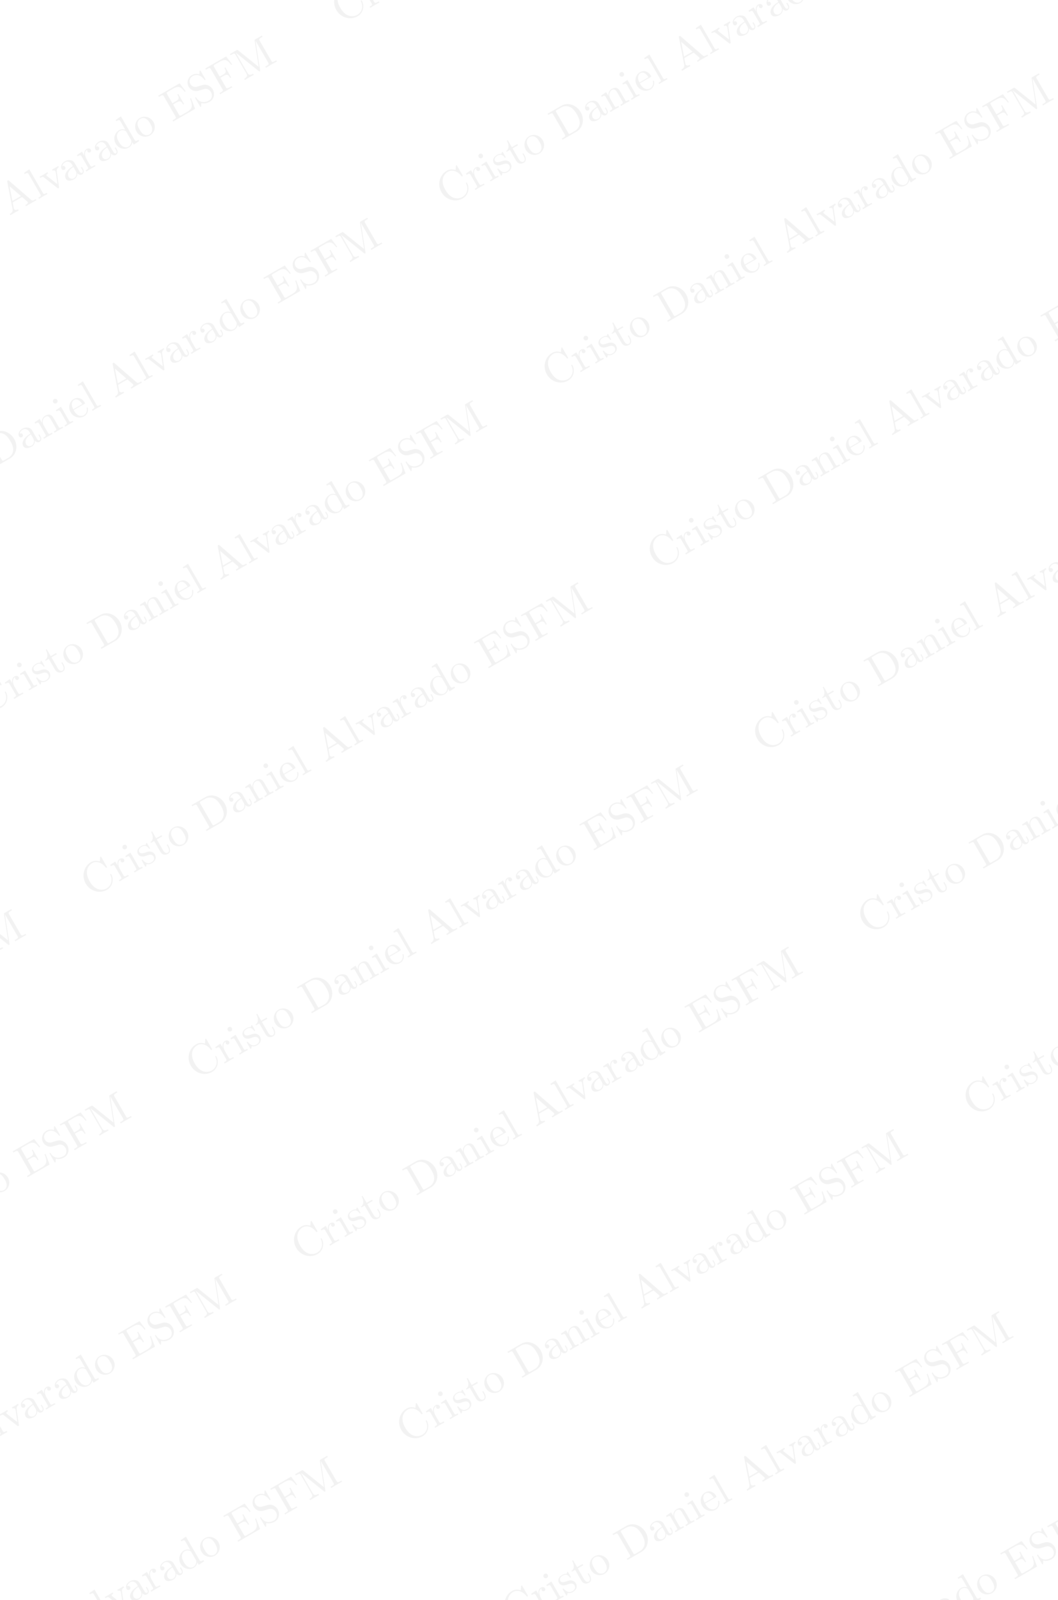
\includegraphics[width=\paperwidth,height=\paperheight,keepaspectratio]{watermark-1.png}
        };
    \end{tikzpicture}
}

% --- Redefiniciones de encabezados de capítulo y sección ---
\makeatletter
% Capítulo (estilo original conservado)
\def\@makechapterhead#1{%
  {\parindent \z@ \raggedright
    \reset@font
    \hrule
    \vspace*{10\p@}%
    \par
    \center \LARGE \scshape \@chapapp{} \huge \thechapter
    \vspace*{10\p@}%
    \par\nobreak
    \vspace*{10\p@}%
    \par
    \vspace*{1\p@}%
    \hrule
    \vspace*{30\p@}  % Espaciado reducido
    \centering\Huge \scshape #1\par\nobreak  % Centrado y scshape
    \vskip 30\p@  % Espaciado reducido
  }}


% Sección
\renewcommand{\section}{\@startsection{section}{1}{\z@}%
  {-2.5ex \@plus -0.5ex \@minus -0.1ex}%  % Espaciado superior reducido
  {1ex \@plus 0.1ex}%                     % Espaciado inferior reducido
  {\normalfont\Large\sectionstyle}}
\newcommand{\sectionstyle}[1]{%
  \par\noindent\hrule
  \vspace{0.2ex}%   % Espaciado entre líneas reducido
  {\scshape{#1}\par}%  % Centrado perfecto y scshape
  \vspace{0.4ex}%   % Espaciado entre líneas reducido
  \hrule
}

% Subsección
\renewcommand{\subsection}{\@startsection{subsection}{2}{\z@}%
  {-2ex \@plus -0.4ex \@minus -0.1ex}%  % Espaciado superior reducido
  {0.8ex \@plus 0.1ex}%                 % Espaciado inferior reducido
  {\normalfont\large\subsectionstyle}}
\newcommand{\subsectionstyle}[1]{%
  \par\noindent\hrule
  \vspace{-0.4ex}%  % Espaciado entre líneas reducido
  {\scshape #1\par}%  % Centrado perfecto y scshape
  \vspace{0.4ex}%  % Espaciado entre líneas reducido
  \hrule
}

% Subsubsección
\renewcommand{\subsubsection}{\@startsection{subsubsection}{3}{\z@}%
  {-1.5ex \@plus -0.3ex \@minus -0.1ex}%  % Espaciado superior reducido
  {0.5ex \@plus 0.1ex}%                   % Espaciado inferior reducido
  {\normalfont\normalsize\subsubsectionstyle}}
\newcommand{\subsubsectionstyle}[1]{%
  \par\noindent\hrule
  \vspace{0.4ex}%   % Espaciado entre líneas reducido
  {\scshape #1\par}%  % Centrado perfecto y scshape
  \vspace{0.4ex}%   % Espaciado entre líneas reducido
  \hrule
}
\makeatother

% --- Entornos personalizados ---
% (aquí puedes definir tus theorems, definiciones, etc.)


% --- Entornos personalizados ---
\newtheoremstyle{largebreak}{}{ }{\normalfont}{}{\bfseries}{}{\newline}{}
\theoremstyle{largebreak}

\newmdtheoremenv[hidealllines=true,roundcorner=5pt,backgroundcolor=gray!60!red!30]{exa}{Ejemplo}[section]
\newmdtheoremenv[hidealllines=true,roundcorner=5pt,backgroundcolor=gray!50!blue!30]{obs}{Observaci\'on}[section]
\newmdtheoremenv[hidealllines=true,roundcorner=5pt,backgroundcolor=green!50!blue!30]{preg}{Pregunta}[section]
\newmdtheoremenv[hidealllines=true,roundcorner=5pt,backgroundcolor=yellow!40]{idea}{Idea}[section]
\newmdtheoremenv[rightline=false,leftline=false]{theor}{Teorema}[section]
\newmdtheoremenv[rightline=false,leftline=false]{propo}{Proposici\'on}[section]
\newmdtheoremenv[rightline=false,leftline=false]{cor}{Corolario}[section]
\newmdtheoremenv[rightline=false,leftline=false]{lema}{Lema}[section]
\newmdtheoremenv[roundcorner=5pt,backgroundcolor=gray!30,hidealllines=true]{mydef}{Definici\'on}[section]
\newmdtheoremenv[roundcorner=5pt]{excer}{Ejercicio}[section]

% --- Comandos auxiliares ---
\def\proof{\paragraph{Demostraci\'on:\\}}
\def\endproof{\hfill$\blacksquare$}
\def\sol{\paragraph{Soluci\'on:\\}}
\def\endsol{\hfill$\square$}

\newcommand\abs[1]{\ensuremath{\left|#1\right|}}
\newcommand\divides{\ensuremath{\bigm|}}
\newcommand\cf[3]{\ensuremath{#1:#2\rightarrow#3}}
\newcommand\contradiction{\ensuremath{\#_c}}
\newcommand\natint[1]{\ensuremath{\left[\big|#1\big|\right]}}

\newcounter{figcount}
\setcounter{figcount}{1}

\renewcommand{\lstlistingname}{Código}
\renewcommand{\lstlistlistingname}{Lista de \lstlistingname s}

% --- Comienzo del documento ---
\begin{document}
    \setlength{\parskip}{5pt}
    \setlength{\parindent}{12pt}
    \title{Machine Learning with PyTorch and Scikit-Learn\\
    
    From Coursera}
    \author{Cristo Daniel Alvarado}
    \maketitle

    \tableofcontents

    \lstlistoflistings

    \newpage

    \chapter{Module 1}

    The goal of this chapter is to explore the foundational concepts of machine learning, focusing on how algorithms can transform data into knowledge. We delve into the practical applications of supervised and unsupervised learning, equipping you with the skills to implement these techniques using Python tools for effective data analysis and prediction.
    
    \begin{obs}[\textbf{Learning Objectives}]
        \textbf{Learning Objectives}:
        \begin{itemize}
            \item Analyze data patterns to make future predictions.
            \item Design systems for supervised and unsupervised learning.
            \item Implement machine learning algorithms using Python tools.
        \end{itemize}
    \end{obs}
        
    \section{Overview}

    The goal basically is to learn machine learning using Python libraries such as Scikit-Learn and PyTorch.

    \section{Giving computers the ability to learn from data}

    So, basically in this scenario we will do the following:
    \begin{itemize}
        \item Implement machine learning algorithms using Python tools.
        \item Desing systems for supervised and unsupervised learning.
        \item Analyze data patterns to make future predictions.
    \end{itemize}

    \section{Introduction}

    \begin{mydef}[\textbf{Machine Learning}]
        \textbf{Machine learning} is the\textit{ application and science of algorithms that make sense of data}.
    \end{mydef}

    The goal of this section is to introduce some of the main concepts and different types of machine learning, together with a basic introduction to the relevant terminology. The goal is to stablish the groundwork for successfully using machine learning techniques for practical prolem solving.

    \subsection{The Three Different Types of Machine Learning}

    In this age, we have a large amount of structured and non-structured data.

    \begin{mydef}[\textbf{Structured and Non-structured Data}]
        \textbf{Structured data} refers \textit{to information that is organized in a predefined format}, typically within a fixed schema, such as rows and columns in a database or spreadsheet

        In contrast, \textbf{non-structured data} \textit{lacks a predefined format or structure and exists in its native, raw state}. It is typically qualitative and encompasses a wide variety of formats such as text documents, emails, social media posts, images, videos, and audio files.
    \end{mydef}

    One of the main goals of machine learning is to extract knowledge from data in order to make predictions.

    \begin{obs}[\textbf{Use of Machine Learning}]
        \textbf{Machine Learning} \textit{offers a more efficient alternative for capturing the knowledge in data to improve the performance of predictive models and make data-driven decisions}.
    \end{obs}
    
    \begin{idea}[\textbf{Note on the use of Machine Learning and some of its Applications}]
        Also, notable progress has been made in medical applications; for example, researchers demonstrated that deep learning models can detect skin cancer with near-human accuracy \href{https://www.nature.com/articles/nature21056}{link to article}.
        
        Another milestone was recently achieved by researchers at DeepMind, who used deep learning to predict 3D protein structures, outperforming physics-based approaches by a substantial margin \href{https://deepmind.com/blog/article/alphafold-a-solution-to-a-50-year-old-grand-challenge-in-biology}{link to article}.  
    \end{idea}
    
    There are three types of machine learning: \textbf{supervised learning}, \textbf{unsupervised learning}, and \textbf{reinforcement learning}. There are fundamental differences between these three types of machine learning and we will look at each of them in detail with some notes on its possible applications.
 
    \begin{longtable}{l p{7cm}}
        \toprule
        \multicolumn{2}{c}{\textbf{Three Types of Machine Learning}} \\
        \midrule
        \endfirsthead
        
        \toprule
        \multicolumn{2}{c}{\textbf{Three Types of Machine Learning}} \\
        \midrule
        \endhead
        
        \bottomrule
        \caption{Three Types of Machine Learning.}
        \label{table:types_machine_learning}
        \endlastfoot
        
        \multirow{3}{*}{Supervised learning} 
        & • Labeled data \\
        & • Direct feedback \\
        & • Predict outcome/future \\
        \hline
        \multirow{3}{*}{Unsupervised learning}
        & • No labels/targets \\
        & • No feedback \\
        & • Find hidden structure in data \\
        \hline
        \multirow{3}{*}{Reinforcement learning}
        & • Decision process \\
        & • Reward system \\
        & • Learn series of actions \\
    \end{longtable}

    \subsection{Supervised Learning}

    The main goal of \textbf{supervised learning} is to \textit{learn a model from labeled training data that allows us to make predicitons about unseen or future data}.

    The term \textit{supervised} refers to a set of training examples (data inputs), where the desired output signals (labels) are already known.

    \begin{mydef}[\textbf{Supervised Learning}]
        \textbf{Supervised learning} is the \textit{process of modeling the relationship between data inputs and the labels}.
    \end{mydef}

    We can think of supervised learning as \textit{label learning}.

    \begin{figure}[h]
        \begin{minipage}{\textwidth}
            \centering
            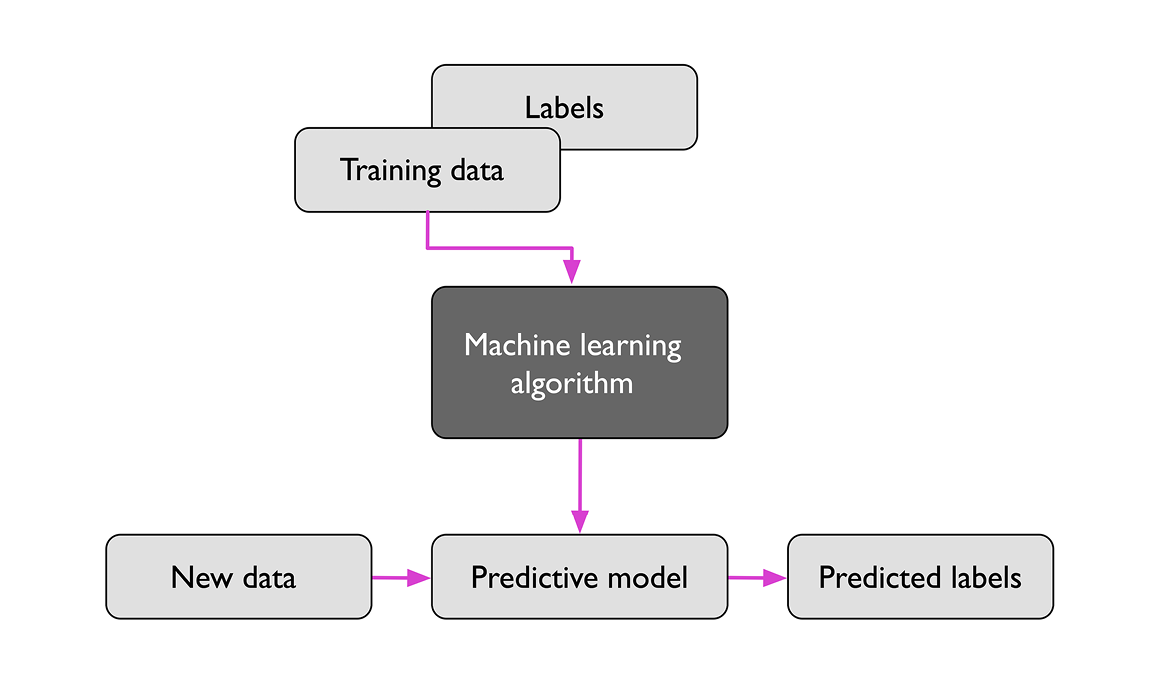
\includegraphics[scale=1]{images/supervised_learning_process.png} \\
            \caption{General Process of Supervised Learning}
            \label{figure:general_process_supervised_learning}
        \end{minipage}
    \end{figure}

    \begin{exa}[\textbf{Example of Supervised Learning}]
        Lets consider the example of email spam filtering. We can train a model using a supervised machine learning algorithm on a corpus of labeled emails, which are correctly marked as spam or non-spam.

        To predict whether a new email belongs to either of the two categories, a supervised learning task with discrete class labels, such as in the previous email spam filtering example.
        
        This is called a \textbf{classification task}. Another subcategory of supervised learning is \textbf{regression}, where the outcome signal is a continous value.
    \end{exa}

    \subsection{Classification for Predicting Class Labels}

    \begin{mydef}[\textbf{Classification}]
        \textbf{Classification} is \textit{a subcategory of supervised learning, where the goal is to predict the categorical class labels of new instances or data points based on past observations}.
    \end{mydef}

    Thos class labels are discrete, unordered values that can be understood as the group memberships of the data points. The previously mentioned example of email spam detection represents a typical example of a binary classification task, where the machine learning algorithm learns a set of rules to distinguish between two possible classes: spam and no-spam emails.

    \begin{figure}[h]
        \begin{minipage}{\textwidth}
            \centering
            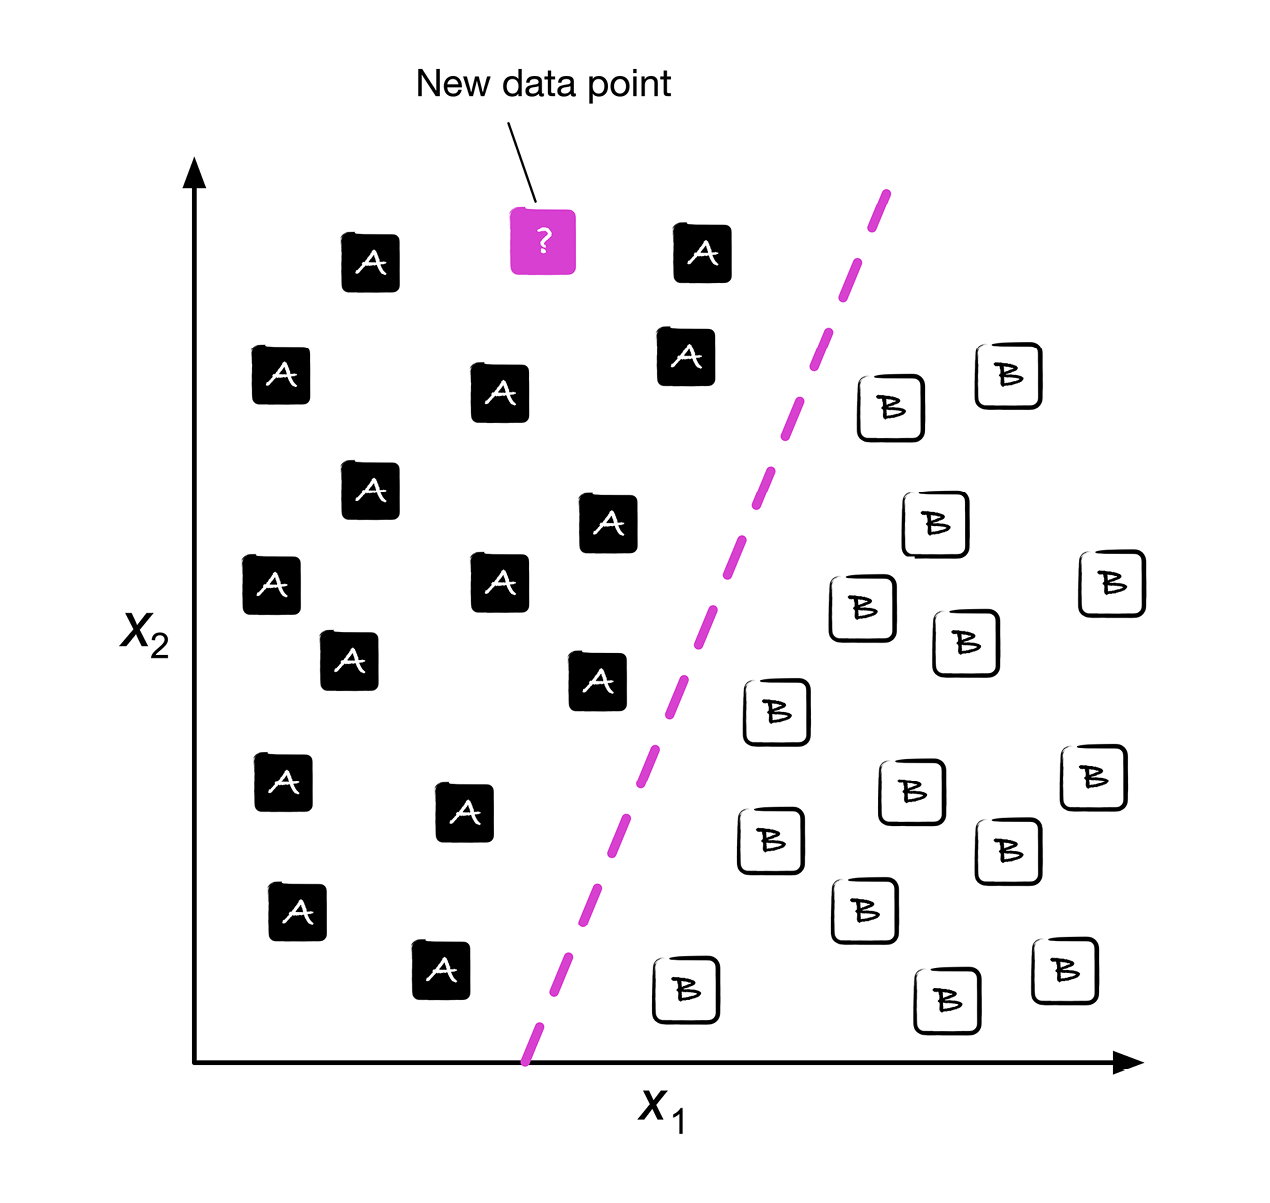
\includegraphics[scale=1]{images/classification_ml} \\
            \caption{Classification in Machine Learning}
            \label{figure:classification_ml}
        \end{minipage}
    \end{figure}

    The next ilustration shows the concept of binary classification task given 30 training examples; 15 training are labeled as \textbf{class A} and the other 15 labeled as \textbf{class B}.

    Our dataset is two-dimensional, meaning that each example has two values associated with it: $x_1$ and $x_2$. We can use a supervised machine learning algorithm to to learn a rule (decision boundary represented as the dashed line) that can separate two classes and classify new data into each of those two categories given its $x_1$ and $x_2$ values.

    \begin{obs}[\textbf{Nature of classification of class labels}]
        When a set of class labels does not have to be of a binar ynature. The predictive model learned by a supervised learning algorithm can assign any class label that was presented in the training dataset to a new, unlabeled data point or instance.
    \end{obs}

    \begin{exa}
        An example of a multiclass classification task is handwritten character recognition.
    \end{exa}

    \subsection{Regression for Predicting Continous Outcomes}

    \begin{mydef}[\textbf{Regression Analysis}]
        In a \textbf{regression analysis}, \textit{we are given a number of predictor (\textbf{explanatory}) variables and a continus response variable (\textbf{outcome}) and we try to finde a relationship between those variables that allows us to predict an outcome}.
    \end{mydef}

    \begin{obs}[\textbf{Feature and Target Variables}]
        In the field of machine learning, the predictor variables are commonly called \textit{features}, and the response variables are referred to as \textit{target variables}.
    \end{obs}

    \begin{exa}
        Let's asume we want to predict the mat SAT scores of students. If there is a relationship between time spent studying for the test and the final scores, we could use it as training data to learn a model that uses the study time to predict the test scores of future students.
    \end{exa}

    Given a feature variable $x$ and a target variable $y$, we fit a straight line to the data points that minimizes the error in predicting $y$ from $x$.

    We can now use the intercept and slope learned from this data to predict the target variable of new data.

    \begin{figure}[h]
        \begin{minipage}{\textwidth}
            \centering
            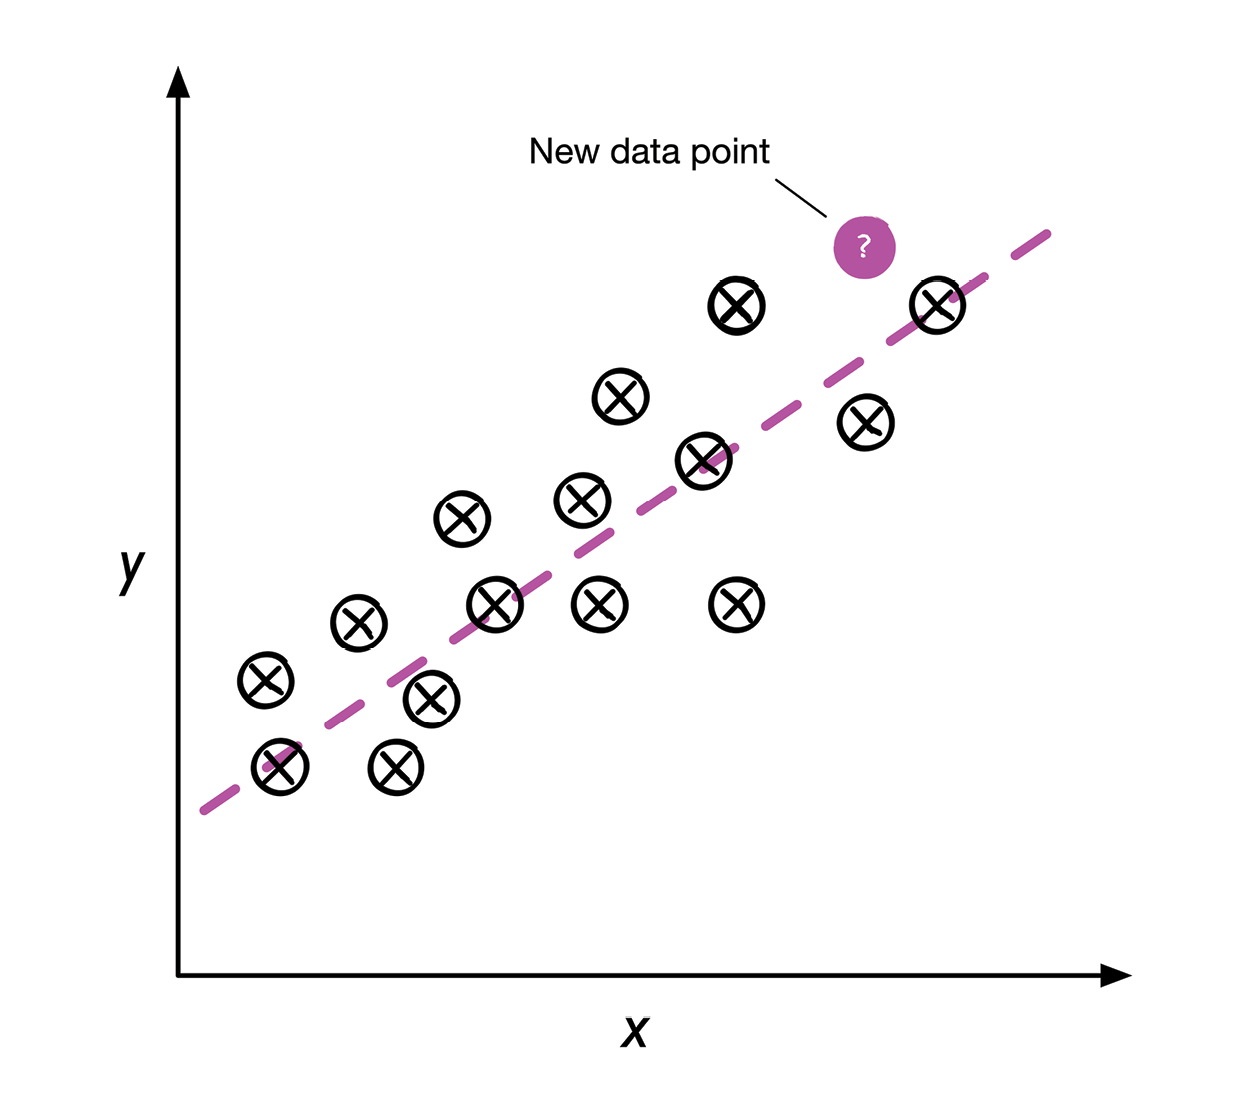
\includegraphics[scale=1]{images/linear_aproximation.png} \\
            \caption{Linear Aproximation}
            \label{figure:linear_aproximation}
        \end{minipage}
    \end{figure}

    
    
\end{document}